%%%%%%%%%%%%%%%%%%%%%%%%%%%%%%%%%%%%%%%%%%%%%%%%%%%%%%%%%%%%%%%%%%%%
%% I, the copyright holder of this work, release this work into the
%% public domain. This applies worldwide. In some countries this may
%% not be legally possible; if so: I grant anyone the right to use
%% this work for any purpose, without any conditions, unless such
%% conditions are required by law.
%%%%%%%%%%%%%%%%%%%%%%%%%%%%%%%%%%%%%%%%%%%%%%%%%%%%%%%%%%%%%%%%%%%%

\documentclass{beamer}
\usetheme[logo=figures/McMasterLogo]{fibeamer}
\usepackage[utf8]{inputenc}
\usepackage[
  main=english, %% By using `czech` or `slovak` as the main locale
                %% instead of `english`, you can typeset the
                %% presentation in either Czech or Slovak,
                %% respectively.
  czech, slovak %% The additional keys allow foreign texts to be
]{babel}        %% typeset as follows:
%%
%%   \begin{otherlanguage}{czech}   ... \end{otherlanguage}
%%   \begin{otherlanguage}{slovak}  ... \end{otherlanguage}
%%
%% These macros specify information about the presentation
\title{Bayesian Networks and Turbo Codes} %% that will be typeset on the
\subtitle{Presented By: Curtis D'Alves} %% title page.
\author{CAS 781}
%% These additional packages are used within the document:
\usepackage{ragged2e}  % `\justifying` text
\usepackage{booktabs}  % Tables
\usepackage{tabularx}
\usepackage{tikz}      % Diagrams
\usetikzlibrary{calc, shapes, backgrounds}
\usepackage{amsmath, amssymb}
\usepackage{url}       % `\url`s
\usepackage{listings}  % Code listings
\usepackage{float}
\usepackage{caption}

\frenchspacing
\begin{document}
  \frame{\maketitle}

  \AtBeginSection[]{% Print an outline at the beginning of sections
    \begin{frame}<beame>r
      \frametitle{Table of Contents}
      \tableofcontents[currentsection]
    \end{frame}}

  \begin{darkframes}
%%%%%%%%%%%%%%%%%%%%%%%%%%%%%%%%%%%%%%%%%%%%%%%%%%%%%%%%%%%%%%%%%%%%%%%%%%%%%%%%%%%%%%%%%%%%%%%%%%%%%%%%%%%%%%%%
%%%%%%%%%%%%%%%%%%%%%%%%%%%%%%%%%%%%%%%%%%%%%%%%%%%%%%%%%%%%%%%%%%%%%%%%%%%%%%%%%%%%%%%%%%%%%%%%%%%%%%%%%%%%%%%%
%%%%%%%%%%%%%%%%%%%%%%%%%%%%%%%%%%%%%%%%%%%%%%%%%%%%%%%%%%%%%%%%%%%%%%%%%%%%%%%%%%%%%%%%%%%%%%%%%%%%%%%%%%%%%%%%

    \section{Conditional Probability Queries}
    \begin{frame}{Conditional Probability Queries}
        
        How do we perform inference over Bayesian Networks? First ask, what are we trying to accomplish \\
        
        \qquad \\
        
        \begin{itemize}
            \item {\bf Evidence:} \alert{$E = e$}
            \item {\bf Query:} subset of variables \alert{$Y$}
            \item {\bf Task:} compute \alert{$P(Y \mid E = e)$}
        \end{itemize}

    \end{frame}

    \begin{frame}{Sum Product}
        
        \begin{figure}
                    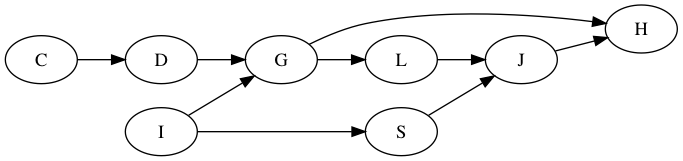
\includegraphics[scale=0.3]{figures/dot_success13}

        \end{figure}

        Assume our goal is to compute \alert{$P(J)$} we only need to eliminate (our marginalize out) all of the variables
  except for \alert{$J$}. So we end up with the following summation over the joint dist. (given using chain rule for BN)        
        \qquad \\
        
            \alert{$ \sum\limits_{C,D,I,G,S,L,H} \phi_C(C) \phi_D(C,D) \phi_I(I) \phi_G(G,I,D) \phi_S(S,I) \phi_J(J,L,S) \phi_H(H,G,J)$}

    \end{frame}
    
    \section{Belief Propagation}
    \begin{frame}{Cluster Graphs}
        
        \begin{figure}
            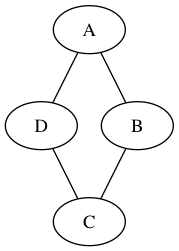
\includegraphics[scale=0.3]{figures/simple_markov}
            \qquad 
            \qquad
            \qquad
            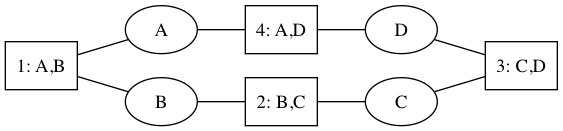
\includegraphics[scale=0.3]{figures/cluster_graph}
            \caption*{Markov Network \qquad \qquad \qquad \qquad \qquad Custer Graph}
        \end{figure}

    Clusters will communicate information via factors \alert{$\phi_1[A,B] \qquad \phi_2[B,C] \qquad \phi_3[C,D] \qquad \phi_4[D,A]$}

    \end{frame}
    
    \begin{frame}{Message Passing}
        \begin{figure}
        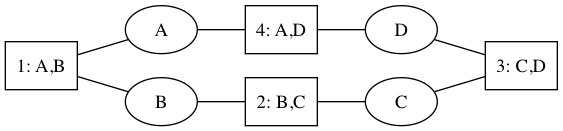
\includegraphics[scale=0.5]{figures/cluster_graph}
        \end{figure}
    
        \begin{itemize}
         \item Clusters are going to pass messages to eachother \alert{$\delta_{i,j}$} between clusters \alert{$i,j$}
         \item Initialize a message between adjacent clusters (say 2 to 1) to be \alert{$\delta_{2,1} = 1$}
         \item Communicate information about \alert{only the variables of concern} through targeted sum products, example: \\
             \alert{$\delta_{1,4} = \sum_B \delta_{2,1}(B) \phi_1(A,B)$}
         \end{itemize}
    \end{frame}

    \begin{frame}{Belief Propagation Algorithm}
        \begin{itemize}
            \item Assign each factor \alert{$\phi_k$} to a cluster \alert{$C_k$}
            \item Construct initial potentials \alert{$\psi_i(C_i) = \Pi_{k:\alpha(k)=i} \phi_k$}
            \item Initialize all messages to be 1
            \item Repeat: for each edge \alert{$(i,j)$} pass message  \\
                \qquad \alert{$\delta_{i,j}(S_{i,j}) = \sum_{C_i-S_{i,j}} \psi_i \times \Pi_{k \in N_i - \{j\}} \delta_{k,j} $}
            \item Compute: \\
                \alert{ $\beta_i(C_i) = \psi_i \times \Pi_{k \in N_i} \delta_{k,i}$}
                
        \end{itemize}

    \end{frame}
  
  \section{Turbo Codes}
  \begin{frame}{Message Coding and Decoding}
      
      \begin{itemize}
          \item Given a message with \alert{k} bits, we wish to transmit over a noisy channel \\
      
          \begin{figure}
            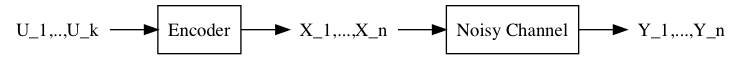
\includegraphics[scale=0.4]{figures/message_code1}
            \qquad 
            \qquad
            \qquad
            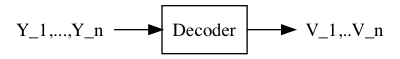
\includegraphics[scale=0.4]{figures/message_code2}
        \end{figure}

        \item Without encoding and decoding, we have no confidence our message was correctly received
    \end{itemize}
  \end{frame}

    \begin{frame}{Turbo Codes: The Idea}
        \begin{figure}
            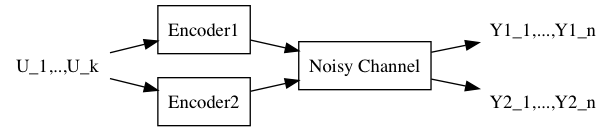
\includegraphics[scale=0.4]{figures/turbo_code1}
        \end{figure}
        
        Compute: \alert{$P(U \mid Y^1, Y^2)$}
        \begin{figure}
            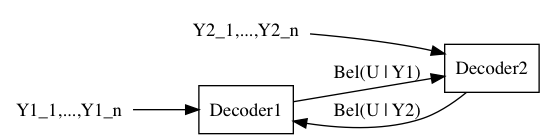
\includegraphics[scale=0.4]{figures/turbo_code2}
        \end{figure}
        \qquad \\
        
        Computed beliefs between decoders are the some as message passing functions \alert{$\delta_{i,j}$}. Hence the algorithm is identical to \alert{Loopy Belief Propagation}
    \end{frame}

  \end{darkframes}

\end{document}
